%package list
\documentclass{article}
\usepackage[top=3cm, bottom=3cm, outer=3cm, inner=3cm]{geometry}
\usepackage{multicol}
\usepackage{graphicx}
\usepackage{url}
%\usepackage{cite}
\usepackage{hyperref}
\usepackage{array}
%\usepackage{multicol}
\newcolumntype{x}[1]{>{\centering\arraybackslash\hspace{0pt}}p{#1}}
\usepackage{natbib}
\usepackage{pdfpages}
\usepackage{multirow}
\usepackage[normalem]{ulem}
\useunder{\uline}{\ul}{}
\usepackage{svg}
\usepackage{xcolor}
\usepackage{listings}
\lstdefinestyle{ascii-tree}{
    literate={├}{|}1 {─}{--}1 {└}{+}1 
  }
\lstset{basicstyle=\ttfamily,
  showstringspaces=false,
  commentstyle=\color{red},
  keywordstyle=\color{blue}
}
%\usepackage{booktabs}
\usepackage{caption}
\usepackage{subcaption}
\usepackage{float}
\usepackage{array}

\newcolumntype{M}[1]{>{\centering\arraybackslash}m{#1}}
\newcolumntype{N}{@{}m{0pt}@{}}


%%%%%%%%%%%%%%%%%%%%%%%%%%%%%%%%%%%%%%%%%%%%%%%%%%%%%%%%%%%%%%%%%%%%%%%%%%%%
%%%%%%%%%%%%%%%%%%%%%%%%%%%%%%%%%%%%%%%%%%%%%%%%%%%%%%%%%%%%%%%%%%%%%%%%%%%%
\newcommand{\itemStudent}{Cristian Raul Saya Vargas, Jean Pier Valera Yana, Cristian Salhua Apfata}
\newcommand{\itemCourse}{Programación}
\newcommand{\itemCourseCode}{20231001}
\newcommand{\itemSemester}{I}
\newcommand{\itemUniversity}{Universidad Nacional de San Agustín de Arequipa}
\newcommand{\itemFaculty}{Facultad de Ingeniería de Producción y Servicios}
\newcommand{\itemDepartment}{Departamento Académico de Ingeniería de Sistemas e Informática}
\newcommand{\itemSchool}{Escuela Profesional de Ingeniería de Sistemas}
\newcommand{\itemAcademic}{2023 - A}
\newcommand{\itemInput}{Del 10 Abril 2023}
\newcommand{\itemOutput}{Al 17 Abril 2023}
\newcommand{\itemPracticeNumber}{05}
\newcommand{\itemTheme}{Django Parte 01}
%%%%%%%%%%%%%%%%%%%%%%%%%%%%%%%%%%%%%%%%%%%%%%%%%%%%%%%%%%%%%%%%%%%%%%%%%%%%
%%%%%%%%%%%%%%%%%%%%%%%%%%%%%%%%%%%%%%%%%%%%%%%%%%%%%%%%%%%%%%%%%%%%%%%%%%%%

\usepackage[english,spanish]{babel}
\usepackage[utf8]{inputenc}
\AtBeginDocument{\selectlanguage{spanish}}
\renewcommand{\figurename}{Figura}
\renewcommand{\refname}{Referencias}
\renewcommand{\tablename}{Tabla} %esto no funciona cuando se usa babel
\AtBeginDocument{%
	\renewcommand\tablename{Tabla}
}

\usepackage{fancyhdr}
\pagestyle{fancy}
\fancyhf{}
\setlength{\headheight}{30pt}
\renewcommand{\headrulewidth}{1pt}
\renewcommand{\footrulewidth}{1pt}
\fancyhead[L]{\raisebox{-0.2\height}{
\includegraphics[width=3cm]{img/logo_episunsa.png}}}
\fancyhead[C]{\fontsize{7}{7}\selectfont	\itemUniversity \\ \itemFaculty \\ \itemDepartment \\ \itemSchool \\ \textbf{\itemCourse}}
\fancyhead[R]{\raisebox{-0.2\height}{
\includegraphics[width=1.2cm]{img/logo_abet}}}
\fancyfoot[L]{Estudiante }
\fancyfoot[C]{\itemCourse}
\fancyfoot[R]{Página \thepage}

% para el codigo fuente
\usepackage{listings}
\usepackage{color, colortbl}
\definecolor{dkgreen}{rgb}{0,0.6,0}
\definecolor{gray}{rgb}{0.5,0.5,0.5}
\definecolor{mauve}{rgb}{0.58,0,0.82}
\definecolor{codebackground}{rgb}{0.95, 0.95, 0.92}
\definecolor{tablebackground}{rgb}{0.8, 0, 0}

\lstset{frame=tb,
	language=bash,
	aboveskip=3mm,
	belowskip=3mm,
	showstringspaces=false,
	columns=flexible,
	basicstyle={\small\ttfamily},
	numbers=none,
	numberstyle=\tiny\color{gray},
	keywordstyle=\color{blue},
	commentstyle=\color{dkgreen},
	stringstyle=\color{mauve},
	breaklines=true,
	breakatwhitespace=true,
	tabsize=3,
	backgroundcolor= \color{codebackground},
}

\begin{document}
	
	\vspace*{10px}
	
	\begin{center}	
		\fontsize{17}{17} \textbf{ Informe de Laboratorio \itemPracticeNumber}
	\end{center}
	\centerline{\textbf{\Large Tema: \itemTheme}}
	%\vspace*{0.5cm}	

	\begin{flushright}
		\begin{tabular}{|M{2.5cm}|N|}
			\hline 
			\rowcolor{tablebackground}
			\color{white} \textbf{Nota}  \\
			\hline 
			     \\[30pt]
			\hline 			
		\end{tabular}
	\end{flushright}	

	\begin{table}[H]
		\begin{tabular}{|x{4.7cm}|x{4.8cm}|x{4.8cm}|}
			\hline 
			\rowcolor{tablebackground}
			\color{white} \textbf{Estudiante} & \color{white}\textbf{Escuela}  & \color{white}\textbf{Asignatura}   \\
			\hline 
			{\itemStudent \par \itemEmail} & \itemSchool & {\itemCourse \par Semestre: \itemSemester \par Código: \itemCourseCode}     \\
			\hline 			
		\end{tabular}
	\end{table}		
	
	\begin{table}[H]
		\begin{tabular}{|x{4.7cm}|x{4.8cm}|x{4.8cm}|}
			\hline 
			\rowcolor{tablebackground}
			\color{white}\textbf{Laboratorio} & \color{white}\textbf{Tema}  & \color{white}\textbf{Duración}   \\
			\hline 
			\itemPracticeNumber & \itemTheme & 04 horas   \\
			\hline 
		\end{tabular}
	\end{table}
	
	\begin{table}[H]
		\begin{tabular}{|x{4.7cm}|x{4.8cm}|x{4.8cm}|}
			\hline 
			\rowcolor{tablebackground}
			\color{white}\textbf{Semestre académico} & \color{white}\textbf{Fecha de inicio}  & \color{white}\textbf{Fecha de entrega}   \\
			\hline 
			\itemAcademic & \itemInput &  \itemOutput  \\
			\hline 
		\end{tabular}
	\end{table}
	
	\section{Tarea}
	\begin{itemize}		
		\item Primeramente creamos nuestro proyecto, con los comando de "django-admin startproject 'nombre del proyecto'"
	\end{itemize}
    \begin{figure}[h]
        \begin{subfigure}{0.5\textwidth}
            \centering
            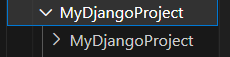
\includegraphics[width=0.9\linewidth]{latex/img/imagen1.png}
            \caption{creacion de proyecto}
            \label{fig:primer}
        \end{subfigure}
    \end{figure}
    \newpage
        \begin{itemize}		
		\item Creandonos la siguiente rama de archivos, junto a nuestro archivo principal el manage.py
            \item Dentro de la subcarptea MyDjangoProject la carpeta de models, donde se guardaran nuestros modelos para nuestra pagina
	\end{itemize}
         \begin{figure}[h]
        \begin{subfigure}{0.5\textwidth}
            \centering
            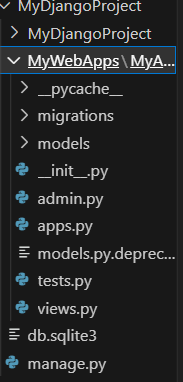
\includegraphics[width=0.5\linewidth]{latex/img/imagen2.png}
            \caption{Rama de archivos creados}
            \label{fig:primer}
        \end{subfigure}
        \begin{subfigure}{0.5\textwidth}
            \centering
            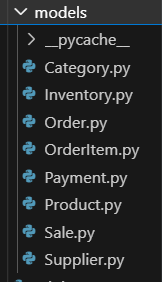
\includegraphics[width=0.5\linewidth]{latex/img/imagen3.png}
            \caption{Modelos creados}
            \label{fig:primer}
        \end{subfigure}
    \end{figure}
    \begin{itemize}		
		\item Category.py : Tenemos nuestro primer modelo el cual representa  la categoria de los productos.
	\end{itemize}
         \begin{figure}[h]
        \begin{subfigure}{0.5\textwidth}
            \centering
            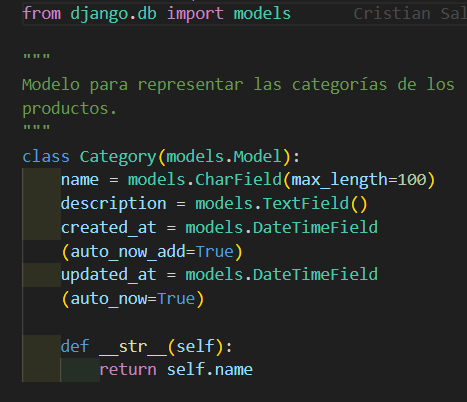
\includegraphics[width=1.03\linewidth]{latex/img/imagen4.png}
            \caption{Category.py}
            \label{fig:primer}
        \end{subfigure}
    \end{figure}
    \newpage
    \begin{itemize}		
		\item Order.py : Modelo que nos representa el orden de las compras
            \item Inventory.py : Modelo que nos representa el inventerio de nuestra pagina
	\end{itemize}
         \begin{figure}[h]
        \begin{subfigure}{0.5\textwidth}
            \centering
            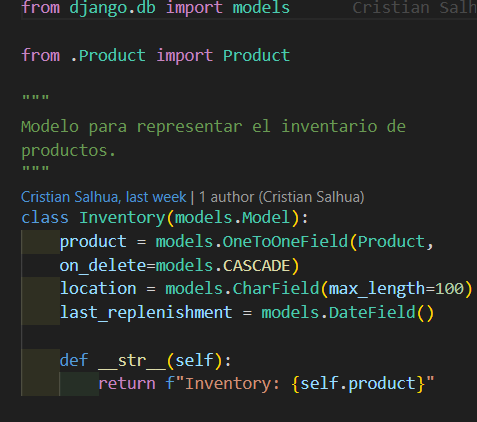
\includegraphics[width=1.03\linewidth]{latex/img/imagen5.png}
            \caption{Inventary.py}
            \label{fig:primer}
        \end{subfigure}
        \begin{subfigure}{0.5\textwidth}
            \centering
            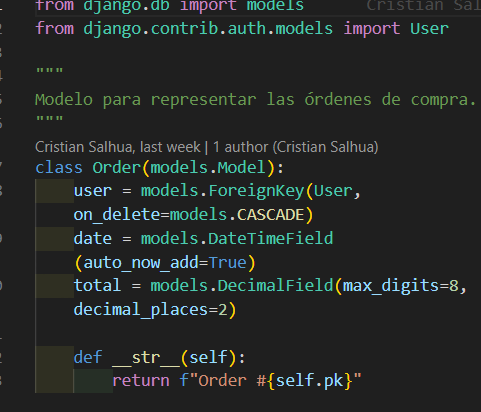
\includegraphics[width=1.03\linewidth]{latex/img/imagen6.png}
            \caption{Order.py}
            \label{fig:primer}
        \end{subfigure}
    \end{figure}
    \begin{itemize}		
		\item OrderItem.py : El siguiente modelo representa el orden de compra de los productos
            \item Paymet.py : El siguiente modelo representa el pago de las ventas
	\end{itemize}
         \begin{figure}[h]
        \begin{subfigure}{0.5\textwidth}
            \centering
            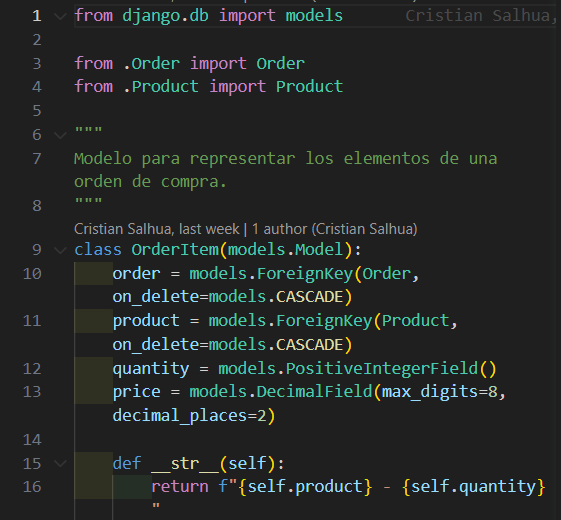
\includegraphics[width=1.1\linewidth]{latex/img/imagen7.png}
            \caption{OrderItem.py}
            \label{fig:primer}
        \end{subfigure}
        \begin{subfigure}{0.5\textwidth}
            \centering
            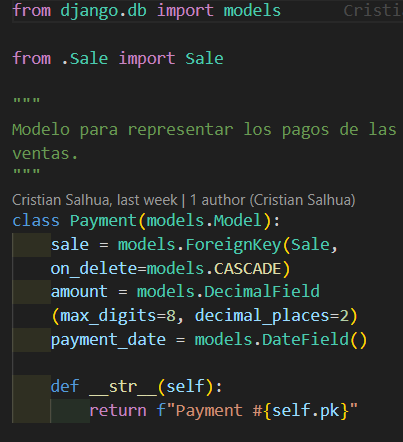
\includegraphics[width=0.9\linewidth]{latex/img/imagen8.png}
            \caption{Paymet.py}
            \label{fig:primer}
        \end{subfigure}
    \end{figure}
    \newpage

    \begin{itemize}		
		\item Product.py : El siguiente modelo representa los productos de nuestra pagina
            \item Sale.py : El siguiente modelo representa las ventas de nuestro producto
	\end{itemize}
         \begin{figure}[h]
        \begin{subfigure}{0.5\textwidth}
            \centering
            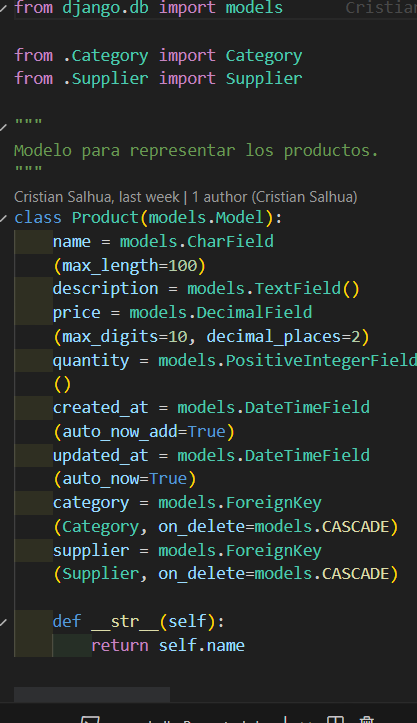
\includegraphics[width=0.8\linewidth]{latex/img/imagen9.png}
            \caption{Product.py}
            \label{fig:primer}
        \end{subfigure}
        \begin{subfigure}{0.5\textwidth}
            \centering
            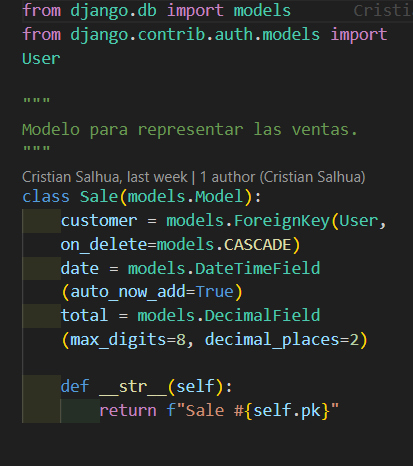
\includegraphics[width=1\linewidth]{latex/img/imagen10.png}
            \caption{Sale.py}
            \label{fig:primer}
        \end{subfigure}
    \end{figure}
    \newpage
    \begin{itemize}		
		\item Supplier.py : Tenemos nuestro ultimo modelo con los datos de proovedores
	\end{itemize}
         \begin{figure}[h]
        \begin{subfigure}{0.5\textwidth}
            \centering
            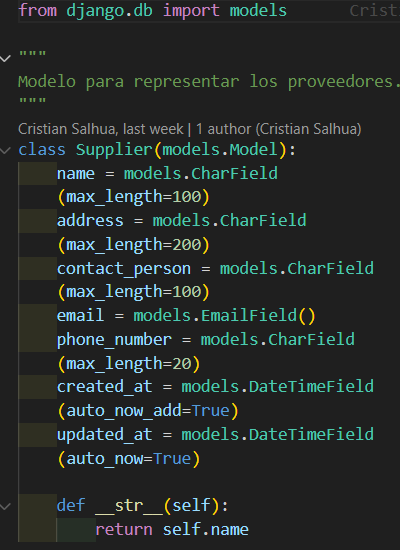
\includegraphics[width=1\linewidth]{latex/img/imagen11.png}
            \caption{Supplier.py}
            \label{fig:primer}
        \end{subfigure}
    \end{figure}
    
		
	\section{Compilacion  }
	\begin{itemize}
		\item Para el proceso de compilamiento tendremos que primero de hacer correr el sistema, para que se nos pueda crear la base de datos que en caso de python usa el SQLITE
		\item Creandonos asi el archibo db.sqlite
		\item Continuando Haremos uso del comando makemigration y el migrate para poder migrar los datos ingresados, los cuales se guardar dentro de la carpeta "migrations"
            \item Finalmente procederemos a compilar llamando al archivo manage.py con el comando "python manage.py runserver
		\Continuaremos 
	\end{itemize}
         \begin{figure}[h]
                \begin{subfigure}{0.5\textwidth}
                    \centering
                    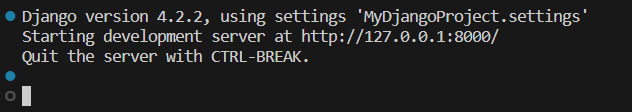
\includegraphics[width=1.5\linewidth]{latex/img/imagen12.png}
                    \caption{link }
                    \label{fig:primer}
                \end{subfigure}
            \end{figure}
            \begin{itemize}
		\item Vemos que nos compila un link el cual se encuentra en el puerto 8000
		\Continuaremos 
	\end{itemize}
        \newpage
        \begin{itemize}
		\item A continuacion nos aparecera la pagina para poder loguearnos, la cual nos mandará a la pagina donde se encuentran los modelos creados
		\Continuaremos 
	\end{itemize}
         \begin{figure}[h]
                \begin{subfigure}{0.5\textwidth}
                    \centering
                    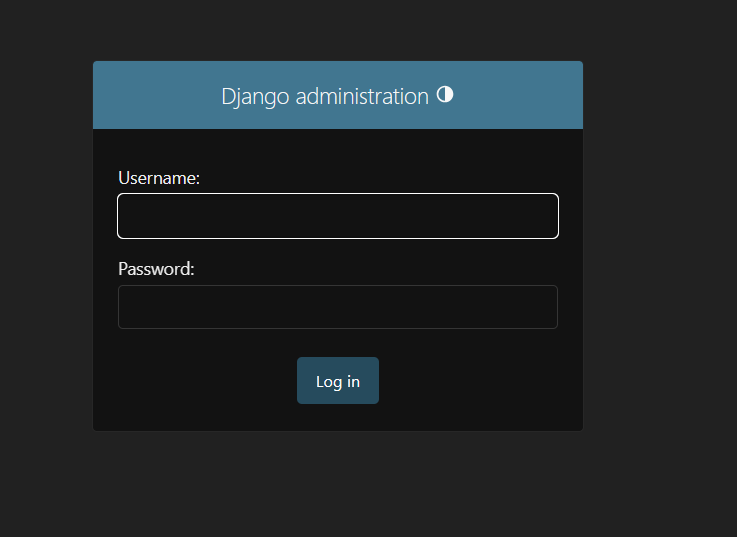
\includegraphics[width=1.2\linewidth]{latex/img/imagen13.png}
                    \caption{Pagina de logueo }
                    \label{fig:primer}
                \end{subfigure}
            \end{figure}
            \begin{itemize}
		\item Nos aparece la pagina con los modelos creados en nuestro proyecto
		\Continuaremos 
	\end{itemize}
         \begin{figure}[h]
                \begin{subfigure}{0.5\textwidth}
                    \centering
                    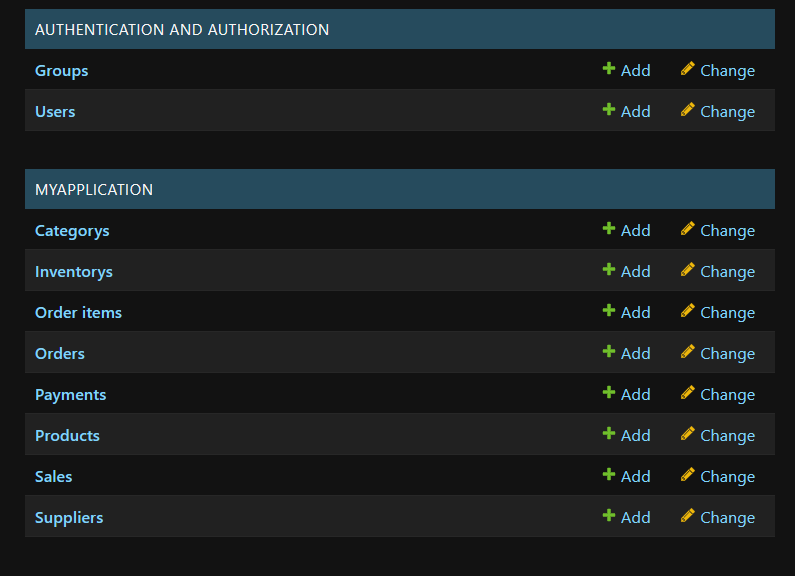
\includegraphics[width=1.2\linewidth]{latex/img/imagen14.png}
                    \caption{Pagina de logueo }
                    \label{fig:primer}
                \end{subfigure}
            \end{figure}
	
	\section{URL de Repositorio Github}
	\begin{itemize}
		\item URL del Repositorio GitHub para clonar o recuperar.
		\item \url{https://github.com/rescobedoq/programacion.git}
		\item URL para el laboratorio 01 en el Repositorio GitHub.
		\item \url{https://github.com/rescobedoq/programacion/tree/main/lab01}
	\end{itemize}
	
\section{PREGUNTA DE APRENDIZAJE}
            \begin{itemize}
		\item (Cristian Roberto Salhua Apfata)
Al estudiar Django, he aprendido la importancia de seguir y cumplir con las convenciones y buenas prácticas de desarrollo de la plataforma. Esto incluye utilizar la estructura de directorios recomendada, aprovechar las funcionalidades y características de Django de manera adecuada, y utilizar la documentación oficial como una guía confiable durante el desarrollo de proyectos. Al seguir estas pautas, se facilita el desarrollo de aplicaciones web, así como la colaboración con otros desarrolladores.
		\item (Cristian Saya Vargas) El Framework Django nos facilita para realizar nuestros proyectos de una manera mas facil ya que nos brinda diferentes herramientas que optimizan el trabajo dando asi tambien la facilidad de realizar dicho proyecto en conjunto sin el riesgo de tener conflictos.
		
		\item (Jeanpier Michaelson Valera Yana)Aprendi a usar nuevas herramientas para el desarrollo con python, un nuevo framkwork que me permitia crear proyectos con una estructura mas amplica y compleja. Al utilizar Django aprendi a relacionar nuevas estructuras dentro y a manejar un sistema diferente entre backend y frontend. Siguiendo instrucciones observe que se crea aplicaciones o productos mucho mas profesionales.
        \item (Christian Henry Venero Guevara)Me ha proporcionado una base sólida para el desarrollo de aplicaciones web, brindando herramientas y estructuras que simplifican muchas tareas comunes. Es importante recordar que hay mucho más por explorar y aprender en Django, ya que es un framework en constante evolución y se pueden desarrollar aplicaciones web aún más complejas y personalizadas con él.
	\end{itemize}
	
	\clearpage
	
	
	

	
		
	\subsection{Estructura de laboratorio 01}
	\begin{itemize}	
		\item El contenido que se entrega en este laboratorio es el siguiente:
	\end{itemize}
	


\section{Pregunta: ¿Cúal es el comportamiento del algoritmo de ordenamiento por inserción?}
	\begin{itemize}
		\item El algoritmo muestra un comportamiento cuadrático de O(n²).
		\item Se trabajarón los peores casos desde una arreglo de tamaño 1 hasta N.
		\item Para obtener un grafico ideal se utilizó N=10,000.
	\end{itemize}		

	\section{\textcolor{red}{Rúbricas}}
	
	\subsection{\textcolor{red}{Entregable Informe}}
	\begin{table}[H]
		\caption{Tipo de Informe}
		{\renewcommand{\arraystretch}{1.5}% for the vertical padding
		\begin{tabular}{|p{3cm}|p{12cm}|}
			\hline
			\multicolumn{2}{|c|}{\textbf{\textcolor{red}{Informe}}}  \\
			\hline 
			\textbf{\textcolor{red}{Latex}} & \textcolor{blue}{El informe está en formato PDF desde Latex,  con un formato limpio (buena presentación) y facil de leer.}   \\ 
			\hline 
			
			
		\end{tabular}
	}
	\end{table}
	
	\clearpage
	
	\subsection{\textcolor{red}{Rúbrica para el contenido del Informe y demostración}}
	\begin{itemize}			
		\item El alumno debe marcar o dejar en blanco en celdas de la columna \textbf{Checklist} si cumplio con el ítem correspondiente.
		\item Si un alumno supera la fecha de entrega,  su calificación será sobre la nota mínima aprobada, siempre y cuando cumpla con todos lo items.
		\item El alumno debe autocalificarse en la columna \textbf{Estudiante} de acuerdo a la siguiente tabla:
	
		\begin{table}[ht]
			\caption{Niveles de desempeño}
			\begin{center}
			\begin{tabular}{ccccc}
    			\hline
    			 & \multicolumn{4}{c}{Nivel}\\
    			\cline{1-5}
    			\textbf{Puntos} & Insatisfactorio 25\%& En Proceso 50\% & Satisfactorio 75\% & Sobresaliente 100\%\\
    			\textbf{2.0}&0.5&1.0&1.5&2.0\\
    			\textbf{4.0}&1.0&2.0&3.0&4.0\\
    		\hline
			\end{tabular}
		\end{center}
	\end{table}	
	
	\end{itemize}
	
	\begin{table}[H]
		\caption{Rúbrica para contenido del Informe y demostración}
		\setlength{\tabcolsep}{0.5em} % for the horizontal padding
		{\renewcommand{\arraystretch}{1.5}% for the vertical padding
		%\begin{center}
		\begin{tabular}{|p{2.7cm}|p{7cm}|x{1.3cm}|p{1.2cm}|p{1.5cm}|p{1.1cm}|}
			\hline
    		\multicolumn{2}{|c|}{Contenido y demostración} & Puntos & Checklist & Estudiante & Profesor\\
			\hline
			\textbf{1. GitHub} & Hay enlace URL activo del directorio para el  laboratorio hacia su repositorio GitHub con código fuente terminado y fácil de revisar. &2 &X &2 & \\ 
			\hline
			\textbf{2. Commits} &  Hay capturas de pantalla de los commits más importantes con sus explicaciones detalladas. (El profesor puede preguntar para refrendar calificación). &4 & & & \\ 
			\hline 
			\textbf{3. Código fuente} &  Hay porciones de código fuente importantes con numeración y explicaciones detalladas de sus funciones. &2 &X &2 & \\ 
			\hline 
			\textbf{4. Ejecución} & Se incluyen ejecuciones/pruebas del código fuente  explicadas gradualmente. &2 &X &2 & \\ 
			\hline			
			\textbf{5. Pregunta} & Se responde con completitud a la pregunta formulada en la tarea.  (El profesor puede preguntar para refrendar calificación).  &2 &X &2 & \\ 
			\hline	
			\textbf{6. Fechas} & Las fechas de modificación del código fuente estan dentro de los plazos de fecha de entrega establecidos. &2 &X &2 & \\ 
			\hline 
			\textbf{7. Ortografía} & El documento no muestra errores ortográficos. &2 &X &2 & \\ 
			\hline 
			\textbf{8. Madurez} & El Informe muestra de manera general una evolución de la madurez del código fuente,  explicaciones puntuales pero precisas y un acabado impecable.   (El profesor puede preguntar para refrendar calificación).  &4 & & & \\ 
			\hline
			\multicolumn{2}{|c|}{\textbf{Total}} &20 & &12 & \\ 
			\hline
		\end{tabular}
		%\end{center}
		%\label{tab:multicol}
		}
	\end{table}
	
\clearpage

\section{Referencias}
\begin{itemize}			
	\item \url{https://www.w3schools.com/java/default.asp}
	\item \url{https://www.geeksforgeeks.org/insertion-sort/}
\end{itemize}	
	
%\clearpage
%\bibliographystyle{apalike}
%\bibliographystyle{IEEEtranN}
%\bibliography{bibliography}
			
\end{document}